\subsection{Real runs analysed individually}\label{sec:c2:real}
For the real runs the measurement errors are unknown, and the candidates were ranked by the profile-likelihood criterion of Eq.~\eqref{eq:bic_profile} with one error standard deviation per species. Table~\ref{tab:c2real} and Fig.~\ref{fig:c2weights} summarise the selection and Fig.~\ref{fig:c2real} shows the fits. Each run was analysed in \BCfifteenMinutes--\BCtwelveMinutes\,min, with the candidates refined in parallel.

\begin{table*}[width=\textwidth,cols=9,pos=t]
\caption{Case study 2, real runs: number of measurements, selected mechanism and shortlist (BIC weights in parentheses), residual standard deviations of the selected mechanism [g\,L$^{-1}$], and BIC difference between the best symbolic-regression law and the selected mechanism (negative: the proposed law is preferred).}\label{tab:c2real}
\begin{tabular*}{\tblwidth}{@{}LCLLCCCCC@{}}
\toprule
Analysis & $n$ & Selected & Shortlist & $X$ & $S_1$ & $S_2$ & $P$ & $\Delta\BIC_{\mathrm{SR}}$ \\
\midrule
\inputtab{generated/tab_c2_real.tex}
\bottomrule
\end{tabular*}
\end{table*}

\begin{figure}
\centering
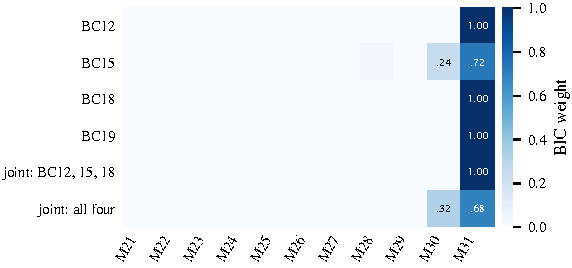
\includegraphics[width=\linewidth]{figs/c2_real_weights.pdf}
\caption{Case study 2, real runs: BIC weights of the eleven library mechanisms for each run analysed alone and for the joint analyses.}
\label{fig:c2weights}
\end{figure}

\begin{figure*}
\centering
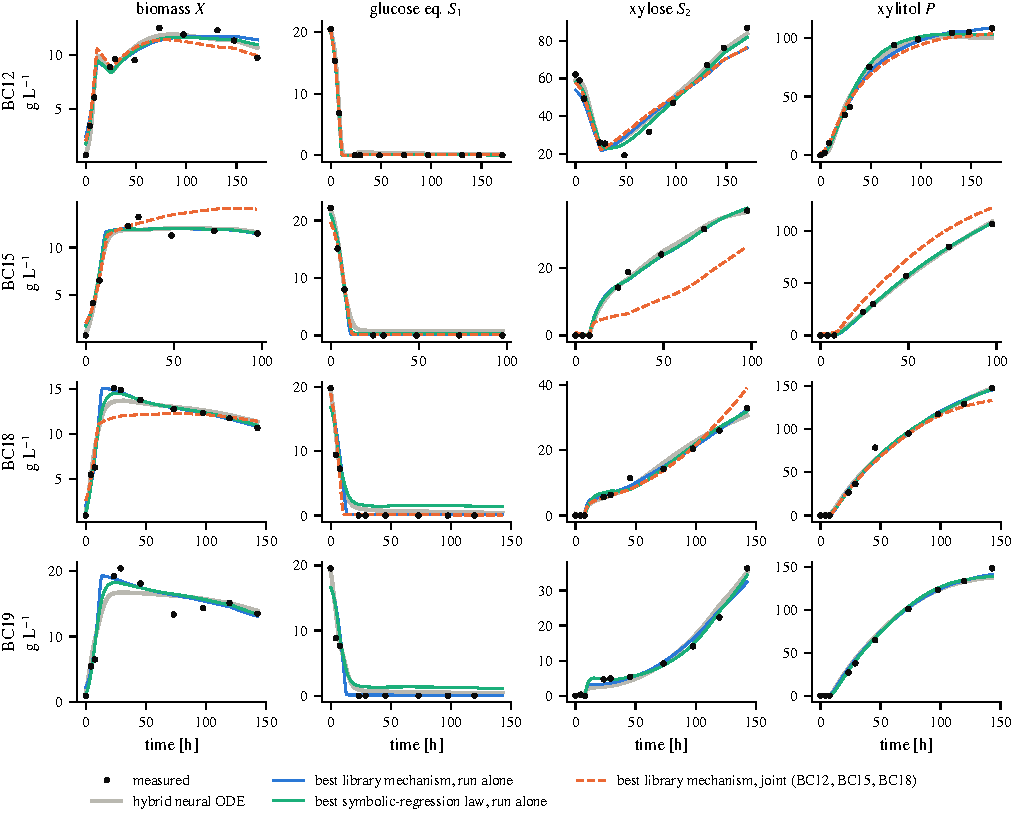
\includegraphics[width=\textwidth]{figs/c2_real.pdf}
\caption{Case study 2, real runs BC12, BC15, BC18 and BC19 (rows): measurements, hybrid neural ODE, best library mechanism and best symbolic-regression law fitted to each run alone, and best library mechanism fitted to BC12, BC15 and BC18 jointly.}
\label{fig:c2real}
\end{figure*}

M31 was selected for every run, with a weight of \BCtwelveW{} for BC12, \BCeighteenW{} for BC18 and \BCnineteenW{} for BC19, and \BCfifteenW{} for BC15, where M30, the same mechanism without death, took most of the remaining weight. The four runs therefore agree on the qualitative mechanism: xylitol formation slows down because both xylose and xylitol inhibit it, and the biomass declines through first-order death during the long production phase. It is consistent with the hybrid model, which learned death rates of 0.013--0.020\,h$^{-1}$ and a conversion rate that declines during the feed phase in BC12, BC18 and BC19 and stays nearly constant in BC15. The residual standard deviations are 1--10\,\% of the ranges of the measured species, with two systematic deviations visible in Fig.~\ref{fig:c2real}. First, the fitted initial biomass exceeds the first measurement by \BCtwelveDXzero, \BCfifteenDXzero, \BCeighteenDXzero{} and \BCnineteenDXzero\,g\,L$^{-1}$ in the four runs, close to the bound of the initial states. This is a limitation shared by all candidates: with a single growth substrate, the model cannot represent the batch phase, in which the yeast grows fast on glucose and then more slowly on the ethanol it produced, and it compensates through the initial biomass. Second, in BC12, the only run with xylose in the batch medium, M31 misses the minimum of the xylose concentration by up to 11\,g\,L$^{-1}$.

The parameter values differ between the runs (Table~\ref{tab:c2params}), and several are poorly determined. The constants of the conversion rate trade off against each other: $K_{S_2}$ lies far above the observed xylose concentrations in three runs, while $K_{SI_2}$ varies between 0.3 and 13\,g\,L$^{-1}$; and $K_{S_1}$ reached its upper bound in two runs. The rates implied by the fits are more comparable than the constants: evaluated at a common state ($S_2=30$ and $P=50$\,g\,L$^{-1}$), the conversion rate of the selected mechanism is \BCtwelveMuRef, \BCfifteenMuRef{} and \BCeighteenMuRef\,h$^{-1}$ for BC12, BC15 and BC18, but only \BCnineteenMuRef\,h$^{-1}$ for BC19, the run supplemented with corn steep solids.

\begin{table*}[width=\textwidth,cols=7,pos=t]
\caption{Case study 2: parameters of M31 fitted to each real run alone and to groups of runs jointly with shared parameters.}\label{tab:c2params}
\begin{tabular*}{\tblwidth}{@{}LCCCCCC@{}}
\toprule
Parameter & \inputtab{generated/tab_c2_real_params_head.tex} \\
\midrule
\inputtab{generated/tab_c2_real_params.tex}
\bottomrule
\end{tabular*}
\end{table*}

\subsection{Real runs analysed jointly}\label{sec:c2:joint}
In case study~1, fitting several runs jointly resolved the ambiguity of single runs. That required the runs to share their kinetics, which held by construction. For real runs it is a hypothesis, and it can be tested with the same criterion: the BIC of a joint fit with one set of kinetic parameters is compared with the BIC of separate fits of the same runs, both evaluated with one error standard deviation per species pooled over the runs (Table~\ref{tab:c2shared}). Because the separate fits were obtained with run-specific error weights, their pooled criterion is an upper bound on its optimum, and the comparison is conservative with respect to separate kinetics.

\begin{table}[width=\linewidth,cols=5,pos=t]
\caption{Case study 2: shared versus run-specific kinetics. BIC of M31 fitted jointly with shared parameters minus BIC of M31 fitted to each run separately, both with one error standard deviation per species pooled over the runs (positive: run-specific parameters are preferred); $k$ counts the kinetic parameters.}\label{tab:c2shared}
\begin{tabular*}{\tblwidth}{@{}LCCCC@{}}
\toprule
Runs & $n$ & $k$ shared & $k$ separate & $\Delta\BIC$ \\
\midrule
\inputtab{generated/tab_c2_shared.tex}
\bottomrule
\end{tabular*}
\end{table}

Joint fitting again selected M31: with a weight of \JointThreeW{} for the three runs in yeast extract--peptone medium (BC12, BC15 and BC18) and of \JointFourW{} for all four runs, with M30 taking the rest (Table~\ref{tab:c2real}, Fig.~\ref{fig:c2weights}). The shared parameters, however, do not describe the runs equally well. In the joint fit of BC12, BC15 and BC18, the residual standard deviations of xylose and xylitol in BC15 rise from about 1\,g\,L$^{-1}$ in its individual fit to 9 and 12\,g\,L$^{-1}$ (Fig.~\ref{fig:c2real}, dashed lines), and the fitted initial biomass of the four-run fit lies 1.8--2.9\,g\,L$^{-1}$ above the first measurements, at the bounds of the initial states. Accordingly, run-specific parameters were preferred for every group of runs tested (Table~\ref{tab:c2shared}), with $\Delta\BIC=\SharedThree$ for the three runs in the same medium and $\Delta\BIC=\SharedTwo$ for BC15 and BC18, the two runs with the most similar operation. The real runs therefore share a mechanism but not its parameter values, and the differences are larger than their measurement errors.

This has a direct consequence for the symbolic regression. For the joint analyses the best proposed laws were preferred to M31 beyond the acceptance threshold ($\Delta\BIC=\JointThreeSRdBIC$ and $\JointFourSRdBIC$; Table~\ref{tab:c2sr}). Both have the same structure, a Monod-type conversion rate with an additional numerator term that decays exponentially with xylitol and a combined inhibition term $PS_2^2$ in the denominator, and their additional terms may absorb part of the differences between the runs: in the three-run fit, for instance, the exponential term has fallen to 10\,\% at 3\,g\,L$^{-1}$ xylitol and only describes a transient at the start of the feed. A law that wins because the model with shared parameters is misspecified is exactly what the adequacy condition of the acceptance rule is meant to reject; without known measurement errors it cannot be applied, and these laws were not accepted.


\subsection{Symbolic regression on the real runs}\label{sec:c2:sr}
Table~\ref{tab:c2sr} lists the best law proposed by the symbolic regression for each analysis; the joint analyses are discussed in Section~\ref{sec:c2:joint}. For the individual runs no proposed law met the acceptance threshold. For BC12 and BC19 the best proposed law was preferred to M31 ($\Delta\BIC=\BCtwelveSRdBIC$ and $\BCnineteenSRdBIC$), close to but not beyond the threshold, for BC15 the two tie, and for BC18 M31 is clearly better. Moreover, the adequacy condition cannot be evaluated without known measurement errors, so on real data even a law that crossed the threshold would be reported as a candidate for further experiments rather than accepted into the library. The proposed laws nevertheless carry information. For every run they include first-order death and describe the decline of the conversion by exponential rather than hyperbolic product inhibition, $\mu_2\propto e^{-P/K}$ with $K$ between 67 and 313\,g\,L$^{-1}$ xylitol. For BC12 the regression adds strong substrate inhibition, $\mu_2\propto S_2e^{-P/K}/(1+S_2^2/K_I)$, and halves the residual standard deviation of xylose relative to M31 (3.6 against 6.7\,g\,L$^{-1}$; Fig.~\ref{fig:c2real}). And the growth laws proposed for BC18 and BC19 are of first order in the glucose equivalent over the observed range, which, together with $K_{S_1}$ at its upper bound, indicates that growth on the lumped substrate saturates more weakly than the library assumes.

\begin{table*}[width=\textwidth,cols=5,pos=t]
\caption{Case study 2, real runs: best laws proposed by symbolic regression and their BIC difference to the best library mechanism. Concentrations in g\,L$^{-1}$, rates in h$^{-1}$; terms that contribute less than 1\,\% of the numerator or denominator over the measured states are omitted.}\label{tab:c2sr}
\begin{tabular*}{\tblwidth}{@{}LLLCC@{}}
\toprule
Analysis & $\mu_1$ & $\mu_2$ & Death & $\Delta\BIC$ \\
\midrule
\inputtab{generated/tab_c2_real_sr.tex}
\bottomrule
\end{tabular*}
\end{table*}
